\section{Configuration Spaces of Polygonal Chains}
% For any regular polygon, there exists a circle in which that polygon can be circumscribed.
% \subsection{Polygonal Linkages}
% \begin{figure}[!ht]
% \begin{center}
% 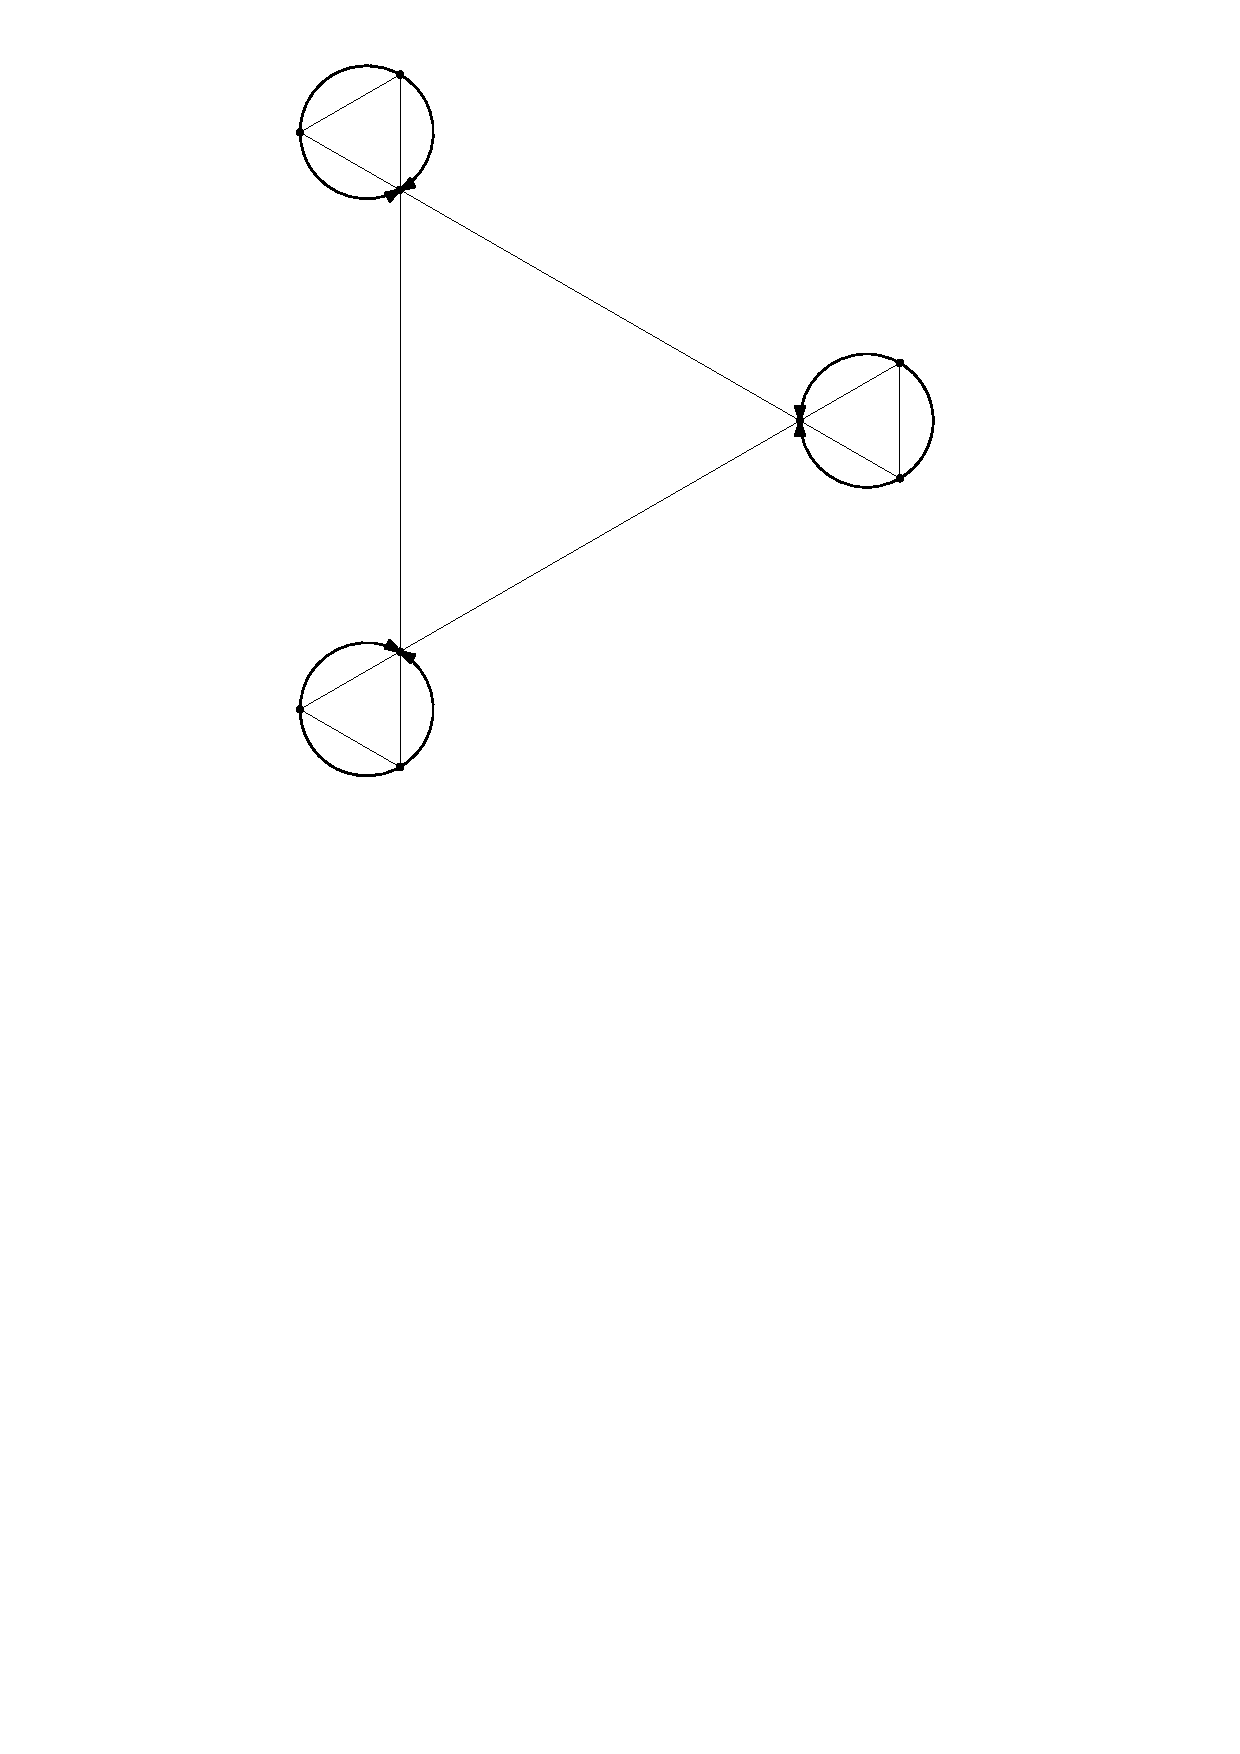
\includegraphics[scale=.5]{graphics/PolygonalLinkageWithConfigurationSpace.pdf}
% \end{center} 
% \caption{\textbf{Not sure how to describe this graph with free joints, pinned joints.  Do I need to define another joint(i.e. axis of rotation joint)?}}
% \end{figure}
% \subsubsection{Configurations and Locked Configurations}
% \subsection{Dissections}
% \begin{prob}[Polygonal Dissection]\label{def:dissection}
% Given two polygons of equal area, $P_1$ and $P_2$, partition $P_1$ into smaller
% pieces,$\left\lbrace P_{1,i}\right\rbrace_{i=1}^n $, rearrange the pieces to
% form $P_2$. \cite{frederickson1997dissections}
% \end{prob}
% \begin{thm}[]\label{thm}
% Any finite collection of polygons of equal area has a common hinged dissection.
% \cite{abbott2012hinged}
% \end{thm}
% \begin{figure}[h]
% \begin{center}
% 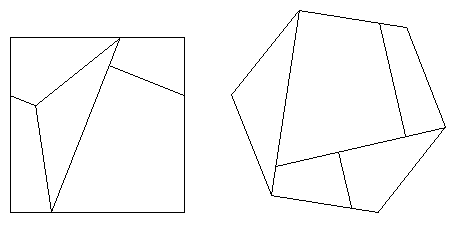
\includegraphics[scale=.3]{graphics/polygonaldissection.png}
% \caption{An axample of two polygons of equal area that can be rearranged into
% the other by the given partition.\cite{davidEppstienJunkyard}}
% \label{fig:polygonaldissection}
% \end{center}
% \end{figure}